%------------------------------------- preamble -------------------------------------
\documentclass{report}

\usepackage{graphicx}
\usepackage{hyperref}
\usepackage{listings}
\usepackage{hyperref}       % to create a linked table of contents


\graphicspath{ {images/} }
\lstdefinestyle{mystyle}{
    breakatwhitespace=false,
    breaklines=true,
    captionpos=b,
    keepspaces=true,
    numbers=left,
    numbersep=5pt,
    showspaces=false,
    showstringspaces=false,
    showtabs=false,
    tabsize=2
}
\lstset{style=mystyle}
\hypersetup{colorlinks,citecolor=black,filecolor=black,linkcolor=black,urlcolor=black}

%------------------------------------- end preamble -------------------------------------
\begin{document}

%-------------------- title -------------------------------------
\title{Sbpy Application Report}
\author{Qingyu Zhang}
\date{June 2021}
\maketitle

\tableofcontents

%--------------------end title --------------------------------

%------------------------------------ chapter 1 -------------------------------------
\chapter{Introduction}

First document. This is a simple example, with no
extra parameters or packages included.

\section{Sbpy}

sbpy is an Astropy affiliated package for small-body planetary astronomy. It is meant to supplement functionality provided by Astropy with functions and methods that are frequently used in the context of planetary astronomy with a clear focus on asteroids and comets\cite{Mommert2019}.

sbpy is motivated by the idea to provide a basis of well-tested and well-documented methods to planetary astronomers in order to boost productivity and reproduceability\cite{Mommert2019}.

\section{Module Structure}
sbpy consists of a number of sub-modules, each of which provides functionality that is tailored to individual aspects asteroid and comet research. The general module design is shown in the following figure \ref{fig:structure}.

\begin{figure}[htb]
    \centering
    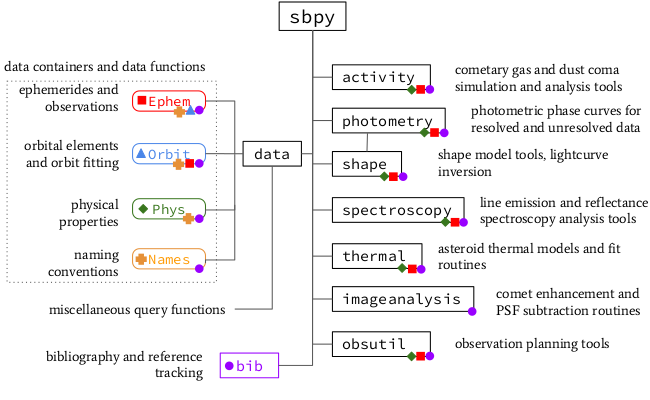
\includegraphics[width=0.5\textwidth]{structure}
    \caption{the module structure of sbpy}
    \label{fig:structure}
\end{figure}

Modules are shown as rectangular boxes, important classes as rounded colored boxes. The left-hand side of the schematic is mainly populated with support modules that act as data containers and query functions. The right-hand side of the schematic shows modules that focus on small body-related functionality. Colored symbols match the colors and symbols of classes and modules they are using.

In our application, we will be using \emph{Ephem} and \emph{Orbit} modules as our data source, then \emph{activity} module to calculate some tasks.

%------------------------------------- end chapter ----------------------------------
%------------------------------------ chapter 2 -------------------------------------
\chapter{Computational Task}
\section{Task1 Orbit}
\subsection{Work Flow}
The first computational task is to compute the orbit of a planet and its position at designated time.
\begin{figure}[htb]
    \centering
    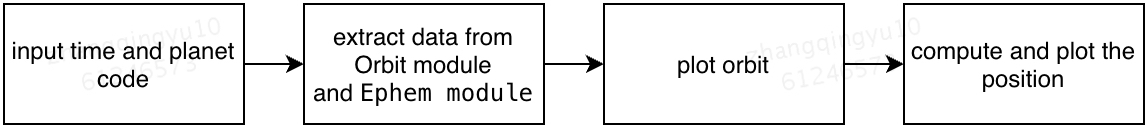
\includegraphics[width=0.8\textwidth]{task1}
    \caption{task2 workflow}
    \label{fig:task2}
\end{figure}

\subsection{User Input}
The application needs user to input the information of the comet or planet including target-id, target-type and so on. Users can get these information through \url{https://ssd.jpl.nasa.gov/horizons.cgi#top}
\subsection{Data Extraction}
Take the default input as an example, we want to plot the orbit of the \emph{46P}, \emph{Earth} and \emph{Jupiter}.
Part of the Orbit data and filed names are shown blow.
\begin{figure}[htb]
    \centering
    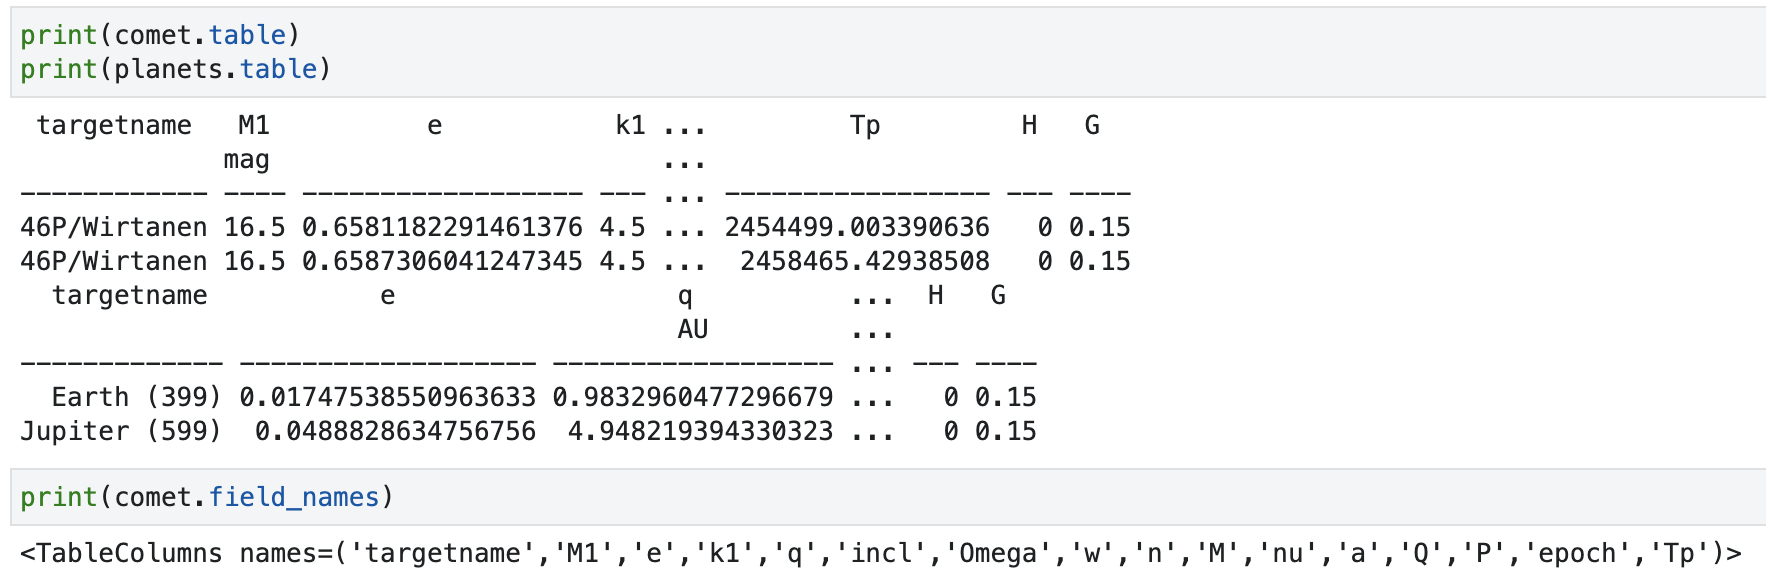
\includegraphics[width=0.5\textwidth]{DataExtraction}
    \caption{Orbit Data}
    \label{fig:OrbitData}
\end{figure}


\subsection{Computation and Visualization}
Code below demonstrates the core of the orbit plotting
\begin{lstlisting}[language=Python]
epochs = orb['epoch'] + np.linspace(-1, 1, 1000) * orb['P'] / 2
eph = Ephem.from_oo(orb, epochs=epochs, dynmodel='2')
ax.plot(eph['x'].value, eph['y'].value, **plot_kwargs)
\end{lstlisting}
After running the program we will get the orbit plot below.
From the outside to the inside, the orbits of Jupiter, comet, and Earth respectively.
\begin{figure}[htb]
    \centering
    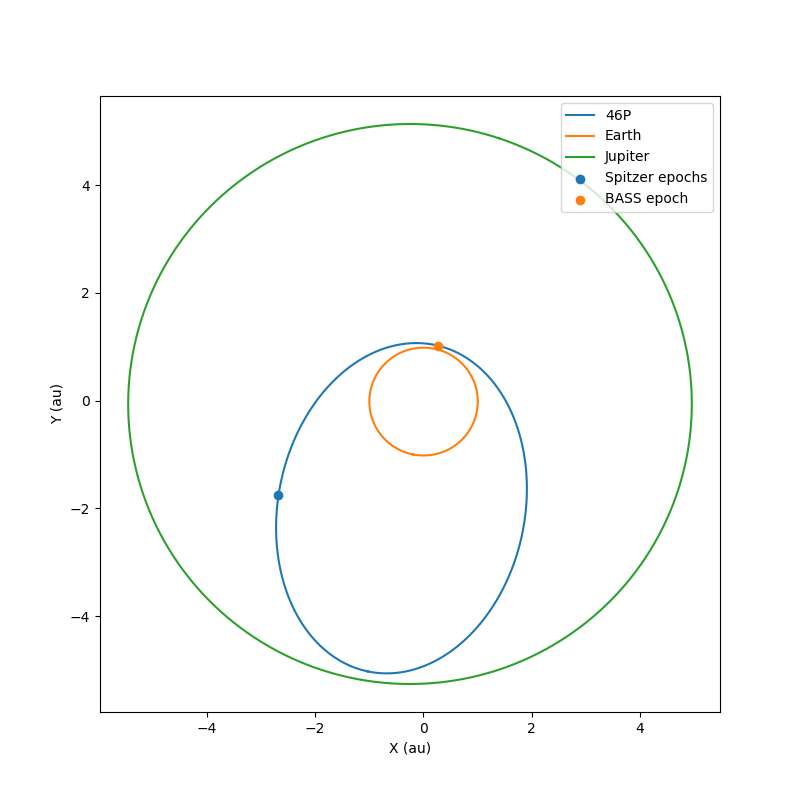
\includegraphics[width=0.5\textwidth]{orbit}
    \caption{Orbit Plot}
    \label{fig:OrbitPlot}
\end{figure}

\section{Task2 Haser Model}
The Haser (1957) model calculates the spatial distribution of coma molecules under photolysis

\subsection{Work Flow}
\begin{figure}[htb]
    \centering
    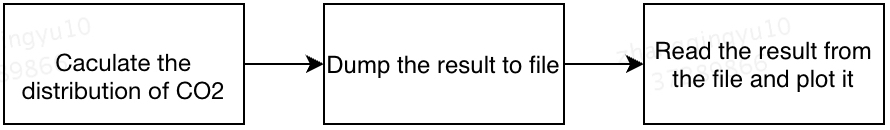
\includegraphics[width=0.7\textwidth]{task2.png}
    \caption{Haser model work flow}
    \label{fig:haser_workflow}
\end{figure}

\subsection{Computation}
Calculate the Haser model column density from 1 to $10^4$ km for CO$_2$, produced at a rate of $10^{28}$/s. Let the expansion velocity be 0.8 km/s.
Let the heliocentric distance range from $1au$ to $10^{11}au$.
Code blow shows the computation of the model.
\begin{lstlisting}[language=Python]
gamma = v * tau * (rh / u.au)**2
co2 = gas.Haser(Q, v, gamma)
\end{lstlisting}

Then save the result object using pickle.
\begin{lstlisting}[language=Python]
with open('haser_ds', 'wb') as f:
    pk.dump(res, f)
\end{lstlisting}

\subsection{Visualization}
First We read the result
\begin{lstlisting}[language=Python]
with open('haser_ds', 'rb') as f:
    res = pk.load(f)
rho = res['rho']
data = res['data']
\end{lstlisting}

Figure blow is the plot of the distribution of $CO_2$
\begin{figure}[htb]
    \centering
    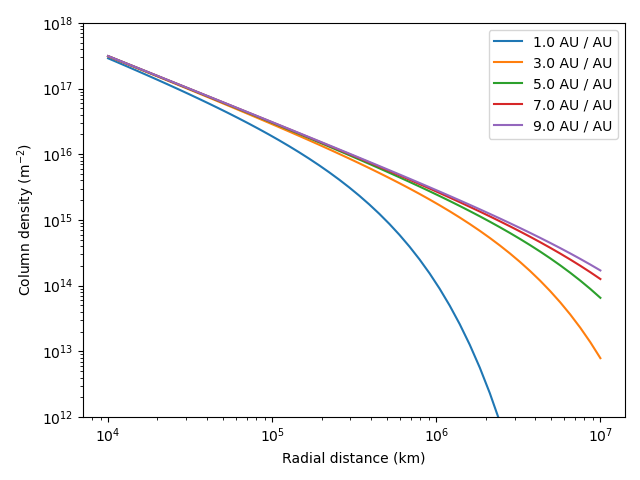
\includegraphics[width=0.8\textwidth]{haser}
    \caption{Distribution of $CO_2$}
    \label{fig:haser}
\end{figure}

%------------------------------------- end chapter ----------------------------------

%------------------------------------ chapter 3 -------------------------------------
\chapter{Conclusion}
Sbpy is an useful package to assist researchers to handle observation data and manipulate them.
It also supply many modules other than data, which is quite difficult for me to understand their application. I used the data module and the activity module, it broadened my field of vision, I've never had a chance to touch professional Astronomy data, fresh but difficult.

Most Importantly, it helps me getting more familiar with those techniques and tools learned from this course.

%------------------------------------ end chapter -------------------------------------
\bibliographystyle{unsrt}
\bibliography{report-bib}

\end{document}